\begin{figure}[H]
	\centering
	\begin{tikzpicture}
		\GraphInit[vstyle=Classic]
		\tikzset{EdgeStyle/.style={->,>=latex}}
		\SetGraphUnit{2}
		%\draw[help lines] (0,0) grid (9,2);
		\Vertex[x=0,y=0,Lpos=-90,L={$f_1$}]{f1}
		\Vertex[x=4.5,y=1,Lpos=-90,L={$f_2$}]{f2}
		\Vertex[x=4.5,y=-1,Lpos=-90,L={$f_{3}$}]{flm1}
		\Vertex[x=9,y=0,Lpos=-90,L={$f_4$}]{fl}
		\Edge[label={$\varrho_{12} \delta_{12} $}](f1)(f2)
		\Edge[label={$\varrho_{13} \delta_{13} $}](f1)(flm1)
		\Edge[label={$\varrho_{24} \delta_{24} $}](f2)(fl)
		\Edge[label={$\varrho_{34} \delta_{34} $}](flm1)(fl)
	\end{tikzpicture}
	\caption{An instance of the alternate hierarchy where \(L=4\) }
	\label{fig:counter_finite}
\end{figure}
